\chapter{Quality Plan}

	\section{Introduction}
	
		The project must comply with all of the requirements described in project requirements specification.  
		The projects conformity to software requirements specification will be checked throughout the lifecycle 
		as defined in the rational unified process. Upon the supervisors verification that all of the tests have 
		been satisfactorily completed / passed, the project is considered to be of satisfactory quality.  
		Meaning that the project complies with all requirements and is accepted by the supervisor.
	
		\begin{figure}[h!]
			\centering
			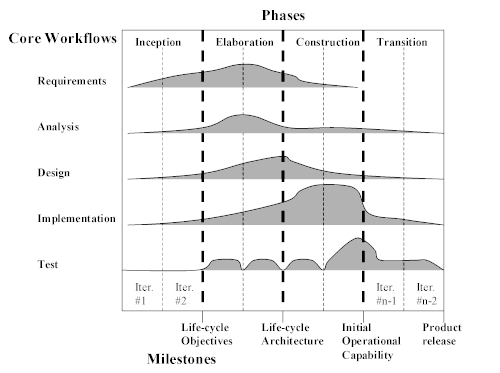
\includegraphics[width=14cm]{figures/rup.jpg}
  			\caption{Rational Unified Process}
		\end{figure}
		
	\section{Review process}
	
		The communications plan outlines the meeting times when software reviews are scheduled to take place.
		The software reviews are in place to detect any defects in the current fidelity prototypes during its construction.  
		The determination of new enhancements, or regressions should be documented and the risk register updated accordingly.
		This should be completed for each of the 4 individual components as outlines in the objectives.  
		\newline
		\newline
		The supervisor in conjunction with the student will attend each review, and critique software prototypes to 
		ensure that the maximum number of possible defects are accounted for, moreover identify risks in the current direction.
		\newline
		\newline
		This review process is subject to the work completed, accounting for disruptions in the work scheduled due to other academic commitments.
		The risk and schedule log should to addressed and adjusted accordingly based upon work interruptions.
		Each meeting will consist of no more than a one hours.  The current	prototype should be provided in advance of this meeting.  
		Any enhancement found to be too difficult or unnecessary for product completion will be noted by the student.
		\newline
	
	\begin{landscape}
		
	\section{Quality Compliancy plan}	
		
	\begin{center}

		\begin{tabular}{ | >{\footnotesize}p{25mm} | >{\footnotesize}p{25mm} | >{\footnotesize}p{35mm} | >{\footnotesize}p{35mm} | >{\footnotesize}p{30mm} | >{\footnotesize}p{17mm} | >{\footnotesize}p{15mm} | >{\footnotesize}p{28mm} | }
			\hline

			  \textbf{Deliverable} 
			& \textbf{Quality Event} 	
			& \textbf{Quality Materials} 
			& \textbf{Quality Metrics} 
			& \textbf{Purpose} 	
			& \textbf{Presenters}
			& \textbf{Validators} 
			& \textbf{Resolution}\\ \hline
			
			
			\rowcolor[gray]{.98}
			  Preliminary Project \newline Conception 												
			& High level \newline Analysis					
			& Project template \newline  Conformance with fyp \newline research expectations	
			& Area of research shows academic value	
			& Compliance with \newline academic expectations \newline prior to submission.
			& Student
			& Supervisor
			& Re-scope project		
			\\ \hline
			
			
			  Project \newline Description \newline Finalization 												
			& Accept project					
			& Academic value 	
			& Timelines and expectations are realistic	
			& Project submittal 
			& Student
			& Supervisor
			& 		
			\\ \hline
			
			
			\rowcolor[gray]{.98}
			  Requirements 												
			& Business \newline modeling \newline Inception					
			& Support for non functional requirements 	
			& Each requirement \newline tracked back to \newline project goal  	
			& Support in \newline Definition scope 
			& Student
			& Supervisor
			& Redefine \newline requirements 		
			\\ \hline
			
			  Scope 												
			& Scope definition \newline Inception					
			& Properly defined scope 	
			& Clearly state whats \newline in / out  	
			& identify clear \newline objectives 
			& Student
			& Supervisor
			& Redefine scope \newline  requirements 		
			\\ \hline
			
			\rowcolor[gray]{.98}
			  Objectives 												
			& Objectives \newline inception					
			& Broken down objectives that realize the scope 	
			& Objective components realize scope  	
			& Define work \newline breakdown structure 
			& Student
			& Supervisor
			& Redefine Objective \newline  scope 		
			\\ \hline
			
			  Work breakdown structure 												
			& Process \newline inception					
			& Each objective broken down 	
			& Clear milestones and finite process   	
			& Define Milestones \newline and schedule
			& Student
			& Supervisor
			& Redefine Objective \newline  scope 		
			\\ \hline
			
			\rowcolor[gray]{.98}
			  Schedule 												
			& Schedule delivery	\newline inception				
			& Timelines or other chart\newline ( gannt ) 	
			& Milestones \newline WBS \newline Dates   	
			& Project progress analysis
			& Student
			& Supervisor
			& Redefine structure \newline  milestones		
			\\ \hline
			
			  Design 												
			& Analysis and \newline design \newline Elaboration					
			& UMl Diagrams 	
			& Class / Sequence \newline diagrams   	
			& Realize requirements
			& Student
			& Supervisor
			&  		
			\\ \hline
			
			\rowcolor[gray]{.98}
			  Test Cases 												
			& Testing \newline Construction					
			& Test harnesses to test business rules  	
			& Code passes tests    	
			& Meet business rules
			& Student
			& Supervisor
			& Redefine design 		
			\\ \hline
			
			  Change Request 												
			& Business rule \newline Conformance					
			& Change request  	
			& Clear \newline requirement change    	
			& Conformance with \newline expectations
			& Supervisor
			& Student
			& Redefine scope \newline  requirements \newline  design 		
			\\ \hline
		
			\rowcolor[gray]{.98}
			  Implementation 												
			& Milestones \newline Construction					
			& Code  	
			& Code passes test cases    	
			& Meet design \newline requirements
			& Student
			& Student
			& Fix bugs 		
			\\ \hline
			
			  Demo 												
			& Deployment					
			& Deployment test harness 	
			& Product realizes \newline requirements    	
			& Show proof \newline of concept
			& Student
			& Supervisor
			&  		
			\\ \hline
			

		\end{tabular}

	\end{center}
	
	\end{landscape}